% !TeX spellcheck = en_US
% !TeX encoding = UTF-8
% !TeX program = pdflatex
% !TeX bib = biber

% ##################################################################################################################
\section{Hamburg Wilhelmsburg}
\label{ch:sc:hhw}
\hfill \textbf{Author:} Hubert Klüpfel and Gregor Lämmel

% ##################################################################################################################
The following describes the evacuation of Hamburg-Wilhelmsburg as a case study. The scenario has been created using MATSim's GRIPS extension package. Technical details about this package are given in Chapter~\ref{ch:evacuation}. 

Wilhelmsburg was severely flooded in 1962. Since then, many structural and operational improvements have been implemented. Back then, the housing situation was rather bad, many people lived in provisional housing due to destruction in World War II. Additionally to the by far more stable buildings, precautions for flooding have been taken and the walls have been heightened. Evacuation is nevertheless necessary under certain circumstances. The relocation of one of the major roads in Wilhelmsburg, the B75, will also influence the evacuation traffic, since it is one of the major north-south arterial roads. In this case study, the consequences of this relocation on the evacuation of Hamburg-Wilhelmsburg is investigated.

% ==================================================================================
\subsection{Brief Description}
The scenario to be investigated here is the relocation of the highway B75 in Wilhelmsburg. Two cases were investigated, as summarized in the following table.
%
\createtable%
	{Scenarios}%
	{Scenarios}%
	{\label{table:b75scenarios}}%
	{%
	\begin{tabular}{|l | l|}
	\hline
	1 & Current location of B75 with restricted directional choice\\
	2 & New location of B75 with restricted locational choice\\
	\hline
\end{tabular}
}%
{}%
%
\createfigure%
	{New and old section of B75}%
	{The current trail of highway B75 is shown in the center of the image. The new trail is east of it close to the railroad.}%
	{\label{fig:overviewB75}}%
	{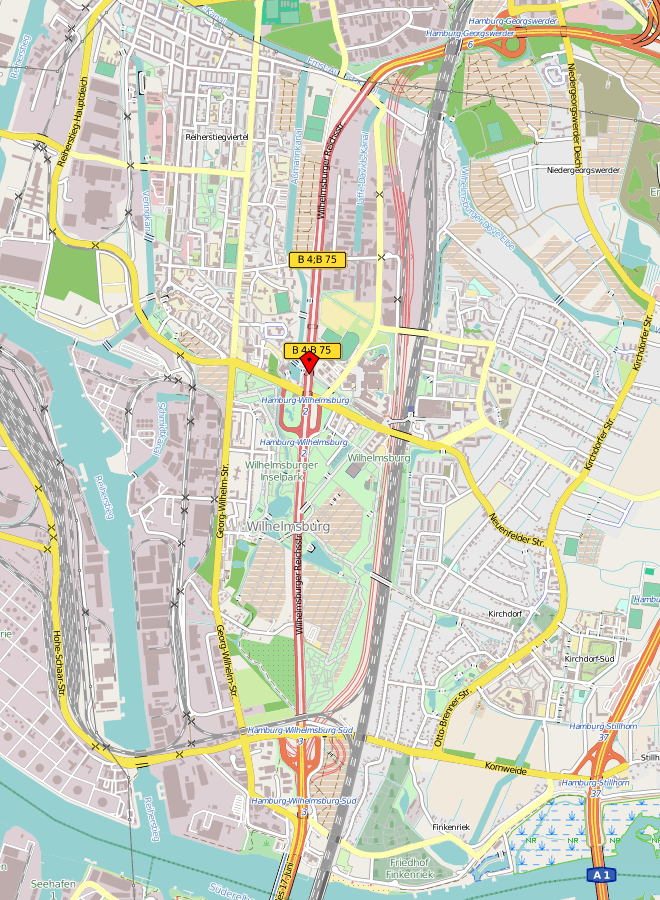
\includegraphics[width=0.7\linewidth]{using/figures/B75overview}}%
{}
%
The aim of the investigation is to highlight differences in the evacuation traffic for both variants of the B75 trail. As can bee seen from Figure~\ref{fig:overviewB75} the new trail "B75 new" is mainly located next to the existing railway track. In the south, the new variant is connected to the existing highway at the junction "Hamburg Wilhelmsburg Süd" (just north of the bridge across the river Elbe) and in the north it is connected to the existing highway just before the junction "Hamburg Georgswerder". The main differences between the two variants are the access to the highway B75 in the center of Wilhelmsburg.

% ==================================================================================
\subsection{Road Network}
The MATSim road network is generated ("imported") from the Hamburg OSM-file. This file was downloaded from \url{www.geofabrik.de}. Fortunately, the osm-file already contains the new track of the B75 highway, marked by an attributed "open 2016". Therefore, the two networks for the variants "B75 old" and "B75 new" can be derived from the same osm-file. For the variant "B75 old" this file can be directly imported. For the variant "B75 new" the part of the B75 that will be relocated, was removed in a first step. In a second step, the new B75 track was connected to the existing road network, i.e.,\,the B75 north at junction "Georgswerder" in the north and junction "Hamburg Wilhelmsburg Süd" in the south.

Additionally, the internal on and off-ramps to the B75 were added. The two variants of the resulting road network, i.e.,\,"B75 old" and "B75 new" are shown in Figure~\ref{fig:b75oldnew}.
%
\createfigure%
{Comparison between network for the old and new track of the B75.}%
{Comparison between network for the old and new track of the B75.}%
{\label{fig:b75oldnew}}%
{%
  \createsubfigure%
  {}%
  {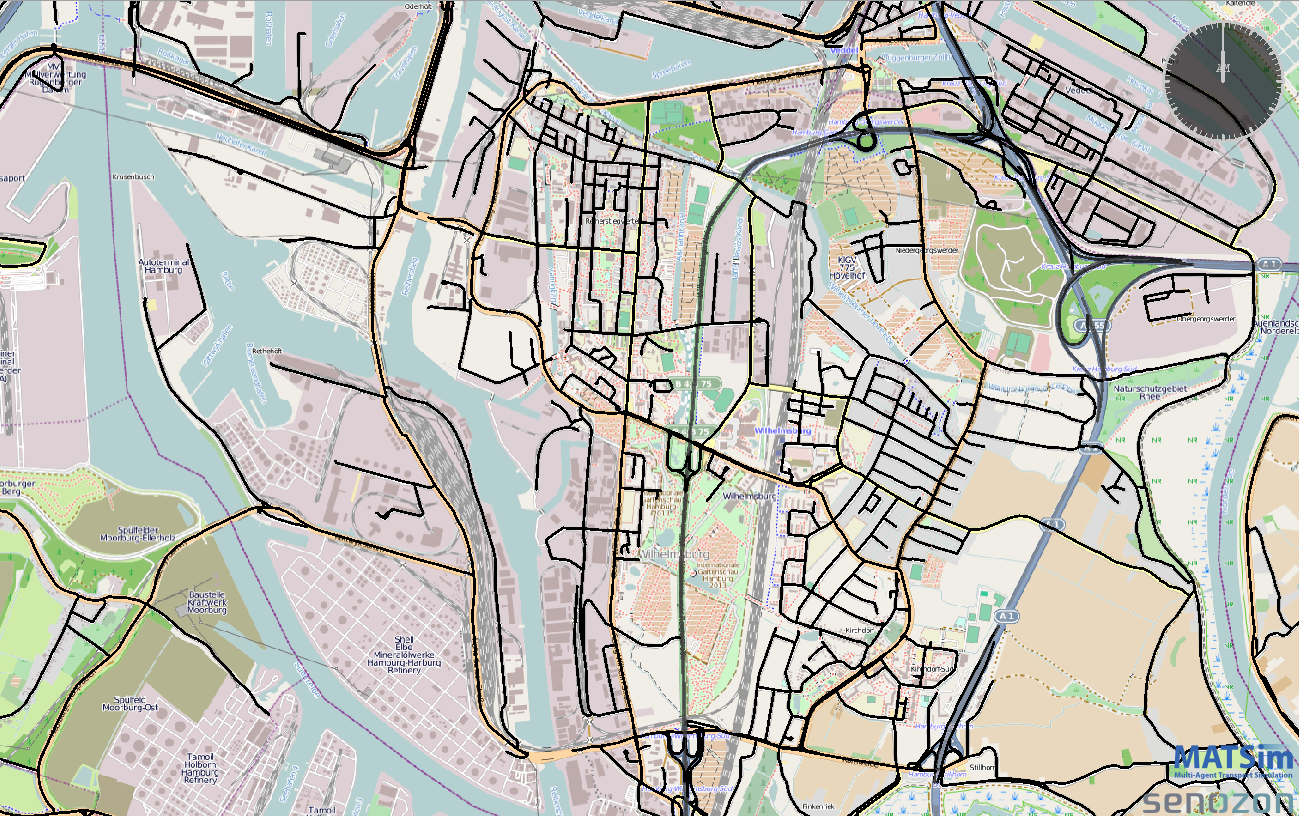
\includegraphics[width=.475\linewidth]{using/figures/B75old}}%
  {}%
  {}%
  \createsubfigure%
  {}%
  {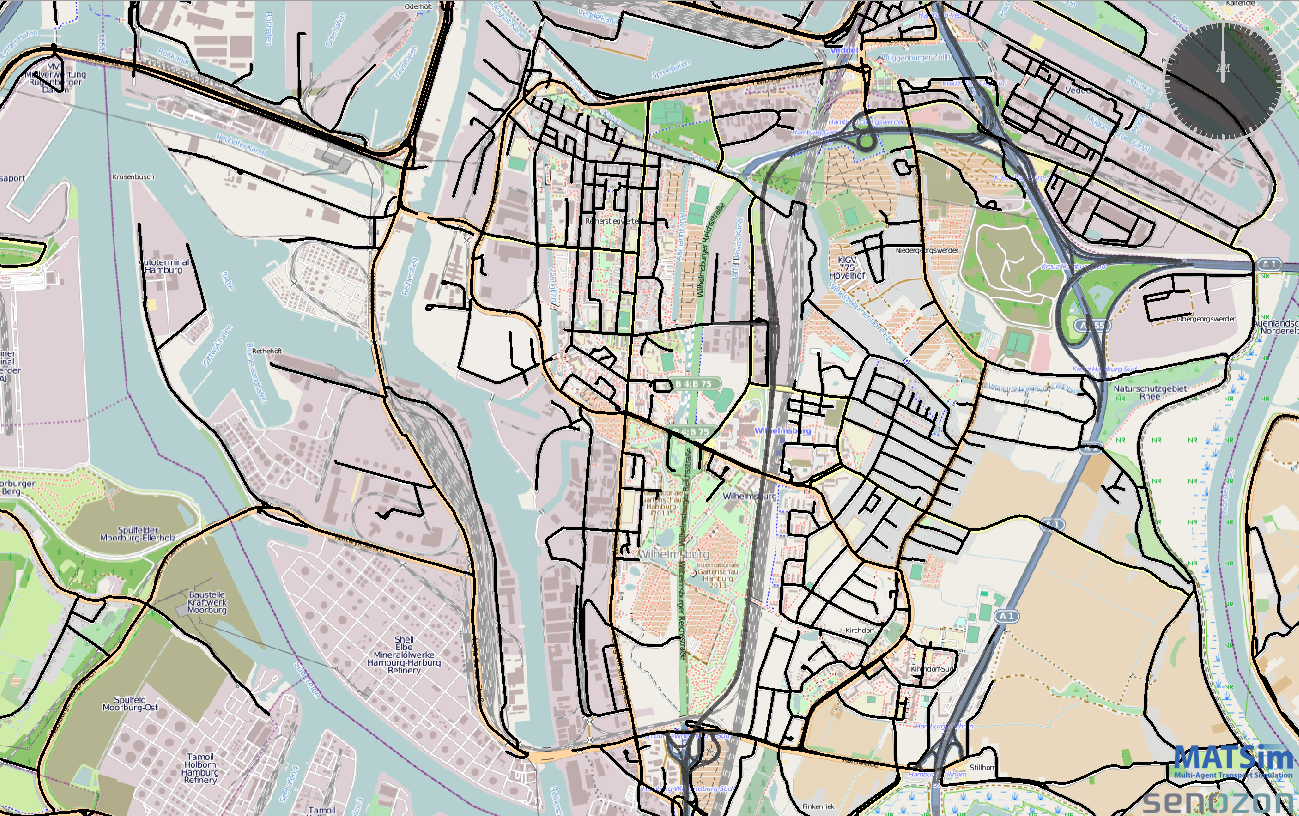
\includegraphics[width=.475\linewidth]{using/figures/B75new}}
  {}%
  {}% 
}%
  {}%

In case of an evacuation, some of the roads will be blocked. The rationale behind this is the avoidance of intersecting traffic. Furthermore, inbound traffic will be blocked, too. The following streets are therefore deleted in the osm file:
%
\begin{itemize}
	\item Neuenfelder Str. 
	\item Im Schönenfelde
	\item Elsterweide
	\item Kirchdorfer Str.
\end{itemize}
%
This is illustrated in Figure~\ref{fig:b75sperrung}.
%
%
\createfigure%
{Closed roads in Hamburg-Wilhelmsburg}%
{Roads closed during evacuation}%
{\label{fig:b75sperrung}}%
{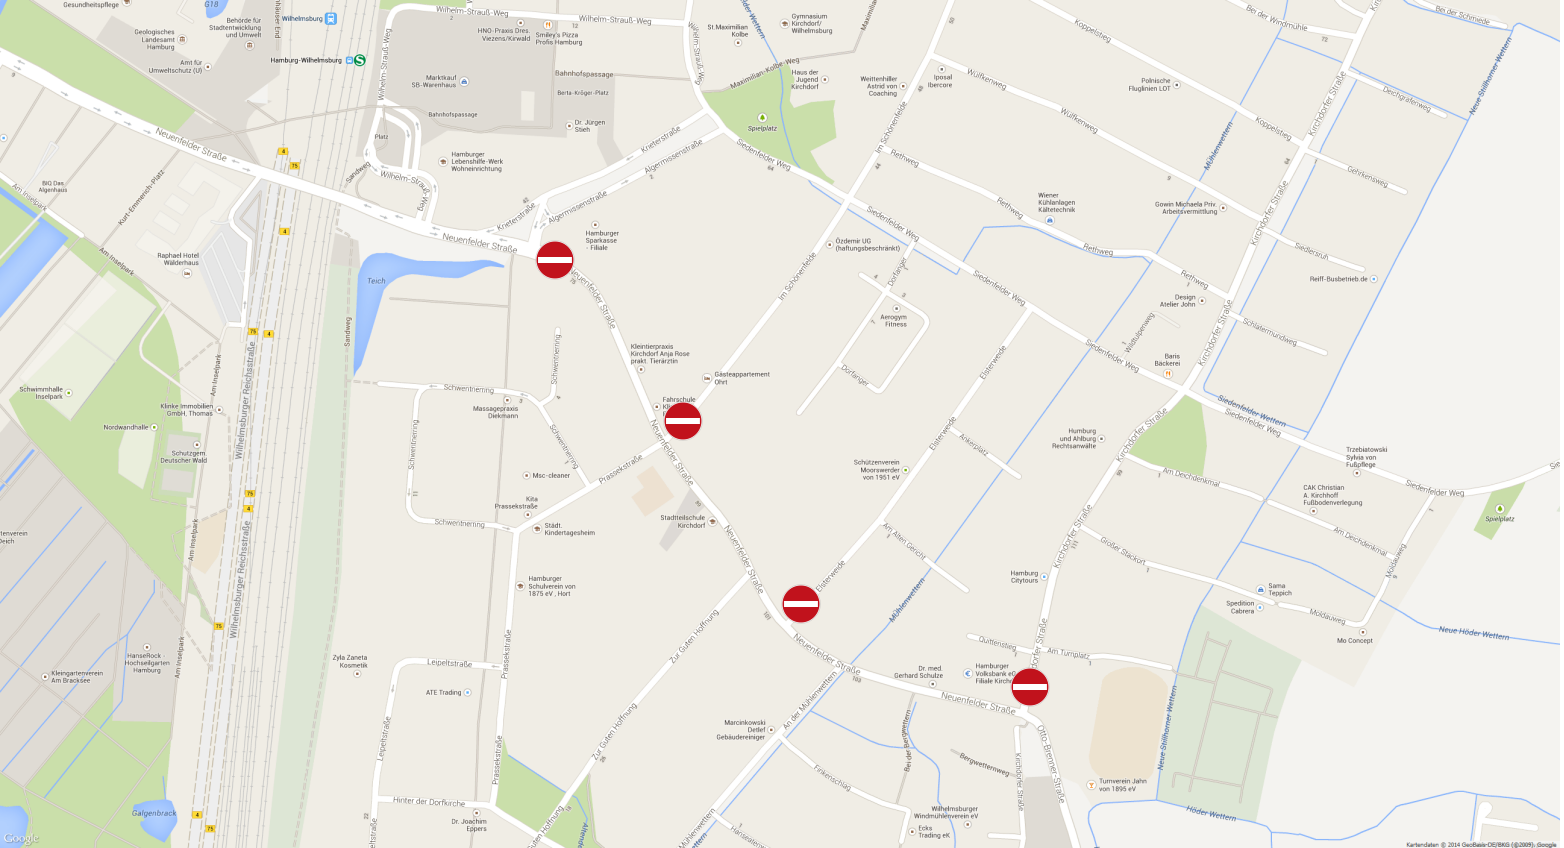
\includegraphics[width=0.7\linewidth]{using/figures/B75sperrung}}%
{}

% ==================================================================================
\subsection{Evacuation Scenario}
The comparison of the two different variants is based on the overall evacuation time, the clearing time of different cells (squares in the area that has to be evacuated), and the numbers of cars using the road network (utilization).

As described in Chapter \ref{evac:section:fifteenminute}, the input files for the network (osm), the area (shp), and the population (shp) as well as the parameters for sample size and departure time distribution can be specified and assessed via a GUI. They are stored in an XML file. The scenario-xml-file for the existing (or "old", in German "alt") track of the B75 highway is shown in the following listing. 

\lstinputlisting[language=XML]{using/scenarios/whb_B75alt.xml}

% ==================================================================================
\subsubsection{Departure Time Distribution}
The departure time distribution is specified in the file scenario.xml. The values are in seconds, i.e.\ a normal distribution with a mean value (mu) and a standard deviation (sigma) of 30 minutes in the range of zero (earliest) to one hour (latest) is chosen. 
More details on the topic of time distributions can be found in Chapter~\ref{chap:evac:eq:mu}. This distribution reflects some assumptions made concerning the evacuation procedure. The overall time frame based on the warning time is 7\,hours at minimum. The preparation phase takes three hours, two hours for setting up the buses and alarming the emergency staff and one hour for the boarding of the buses. The available time for the evacuation is three hours with a buffer of one hour. 
The warning via radio is started at t=0 hrs and the local warning (e.g.,\,by police cars, sirens, and via short messages) at t=1\,hours. Therefore, the reference point for the simulation was set to t=3\,hours. The acceptance criterion for the simulation concerning overall time is the required safe evacuation time (for the sake of the simulation by car) to be less than three hours (including reaction time). The reaction time set in the simulation can therefore be interpreted as a decision making time after having prepared the personal belongings. In short: ASET (available safe evacuation time determined by the flooding) is 3\,hours and the required safe egress time is determined by the simulation. The criterion for a successful evacuation is ASET $>$ RSET.

% ==================================================================================
\subsubsection{Population Size}
As explained previously, the population is not stored in the scenario file but in the population shape file. The reason is that a population file might consist of several polygons. The number of persons is stored an attribute for each polygon. Here, the population size is 11\,924 agents. This number is derived from the number of cars registered in Wilhelmsburg. There is an overall population of approximately 50\,000. One has to take into account the fact, that only part of the population will have to evacuate. For many, it might be sufficient to go to higher places. Detailed information on the different procedures can be found at \url{http://www.hamburg.de/sturmflut/3425646/sturmflut-download-1/} (in German, though).

Each agent represents one evacuee traveling by car. If one would like to check the number of agents by herself based on the simulation files, one can open the file \lstinline|population.dbf| with a database or spreadsheet editor. Note that the number specified in the \lstinline|population.shp| (resp. \lstinline|population.dbf|) will be multiplied with the \lstinline|sampleSize| when converting the files to MATSim input, i.e.,\,in this case the \lstinline|population.xml.gz| located in the output directory.

The population is initially distributed as shown in Figure~\ref{fig:B75initial}. 
%
\createfigure%
{Initial distribution of agents.}%
{The initial distribution of the agents for the evacuation of Wilhelmsburg (for both cases, B75 new and old).}%
{\label{fig:B75initial}}%
{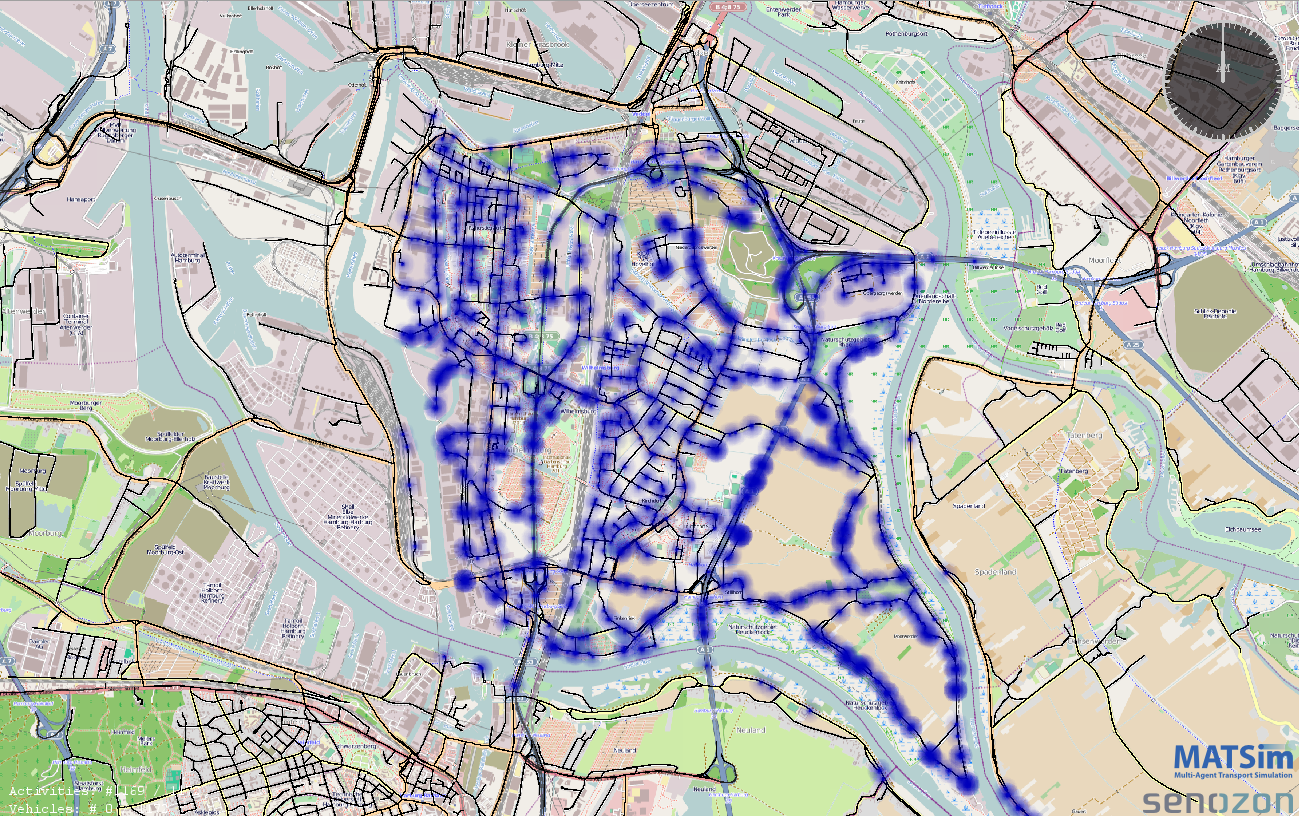
\includegraphics[width=0.7\linewidth]{using/figures/B75initial}}%
{}
The algorithm that converts the area and the population (i.e.,\,\lastinline|area.shp| and \lstinline|population.shp|) is described in Chapter~\ref{chap:evac:fig:area_pop}). It assigns agents to the edges of the network. In the case study, the areas of the harbor were left out and agents were equally distributed to the streets of the housing (and agricultural) areas of Wilhelmsburg (\ Figure~\ref{fig:B75initial}).
This could of course be further refined by going to blocks or even houses and assigning the population according to the detailed statistical housing data. This was not performed for the sake of this simulation, though. The main reason is twofold: Firstly, there are many assumptions concerning the behavior, initial location, and share of population that needs to evacuate. Therefore, the level of detail seems to be sufficient. Secondly, each agent represents a car driver, i.e.,\,in the simulation all the cars registered in Wilhelmsburg leave the area. Taking into account the fact that inbound and through traffic will be prohibited when the level of flooding exceeds a certain threshold, this is a "worst case" assumption leading the a rather heavy traffic load. In summary, the overall approach seems to be justified to assess the relocation of the highway B75 based on a rather heavy traffic load with a reaction time span between 0 and 1\,hour.

% ==================================================================================
\subsection{Simulation Results}
The simulation results are summarized in Table~\ref{table:b75results}. The 0th iteration is based on the shortest distance only. 
%
\createtable%
{Results.}%
{Results.}%\begin{table}[!ht]
%	\centering
%	\caption{Results.}
{\label{table:b75results}}%
{%
\begin{tabular}{|c|c|c|}
	\hline \rule[-2ex]{0pt}{5.5ex}  & B75 old & B75 new \\ 
	\hline \rule[-2ex]{0pt}{5.5ex}  Iteration & Time &  (hh:mm) \\ 
	\hline \rule[-2ex]{0pt}{5.5ex}  00 & 04:45 &  05:00\\ 
	\hline \rule[-2ex]{0pt}{5.5ex}  10 & 01:52 &  01:58\\ 
	\hline \rule[-2ex]{0pt}{5.5ex}  20 & 01:42 &  01:46\\ 
	\hline \rule[-2ex]{0pt}{5.5ex}  30 & 01:40 &  01:42\\ 
	\hline 
\end{tabular}
}%
{}% 
%
This might result in "strange" behavior as illustrated in the following Figure~\ref{fig:B75iteration0}. South of the bridge across the Elbe river, near the junction "Gro{\ss}moordamm". The road network has a circular shape resulting from the fact that it is cut out from the osm road network according to the \lstinline|area.shp|, which is in our case just a circle. Since all the agents are taking the shortest path in iteration 0, they area heading to the closest road out of the evacuation area. Technically, the boundary links in the network are connected to a super link when creating the MATSim network from the osm-file and the \lstinline|area.shp|. This super-link is the destination in all evacuees plans. 
%
\createfigure%
{Results for B75 old, iteration 0}%
{Results for B75 old, iteration 0.}%
{\label{fig:B75iteration0}}%
{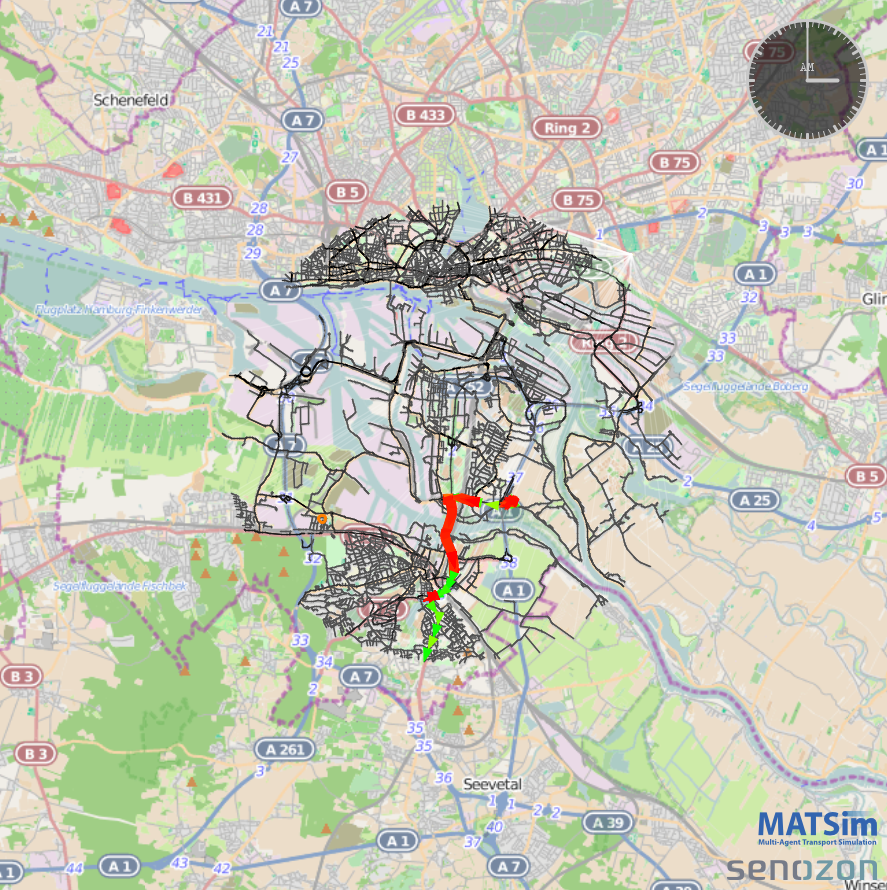
\includegraphics[width=0.7\linewidth]{using/figures/B75iteration0}}%
{}
%
A second factor contributing to the congestion in iteration 0 is a short cut via an on- and off-ramp of the Autobahn A253 at "Gro{\ss}moordamm". The capacity of the on- and off-ramp is 1\,500 cars per hour compared to 4\,000 cars per hour on the highway. Therefore, the short cut (which is shorter in distance, that's the reason why the agents take it) is a bottleneck, resulting in artificial congestion in iteration 0.
Therefore, the 0th iteration is not suitable for assessing the overall evacuation time. As can be seen from table~\ref{table:b75results} above, for both cases, from iteration 10 on the time presumably converges to some realistic value. This is also illustrated in Figure~\ref{fig:B75iteration20} where the situation at t=1:30\,hours is shown for iteration 20.
%
\createfigure%
{Results for B75 old, iteration 20}%
{Results for B75 old, iteration 20.}%
{\label{fig:B75iteration20}}%
{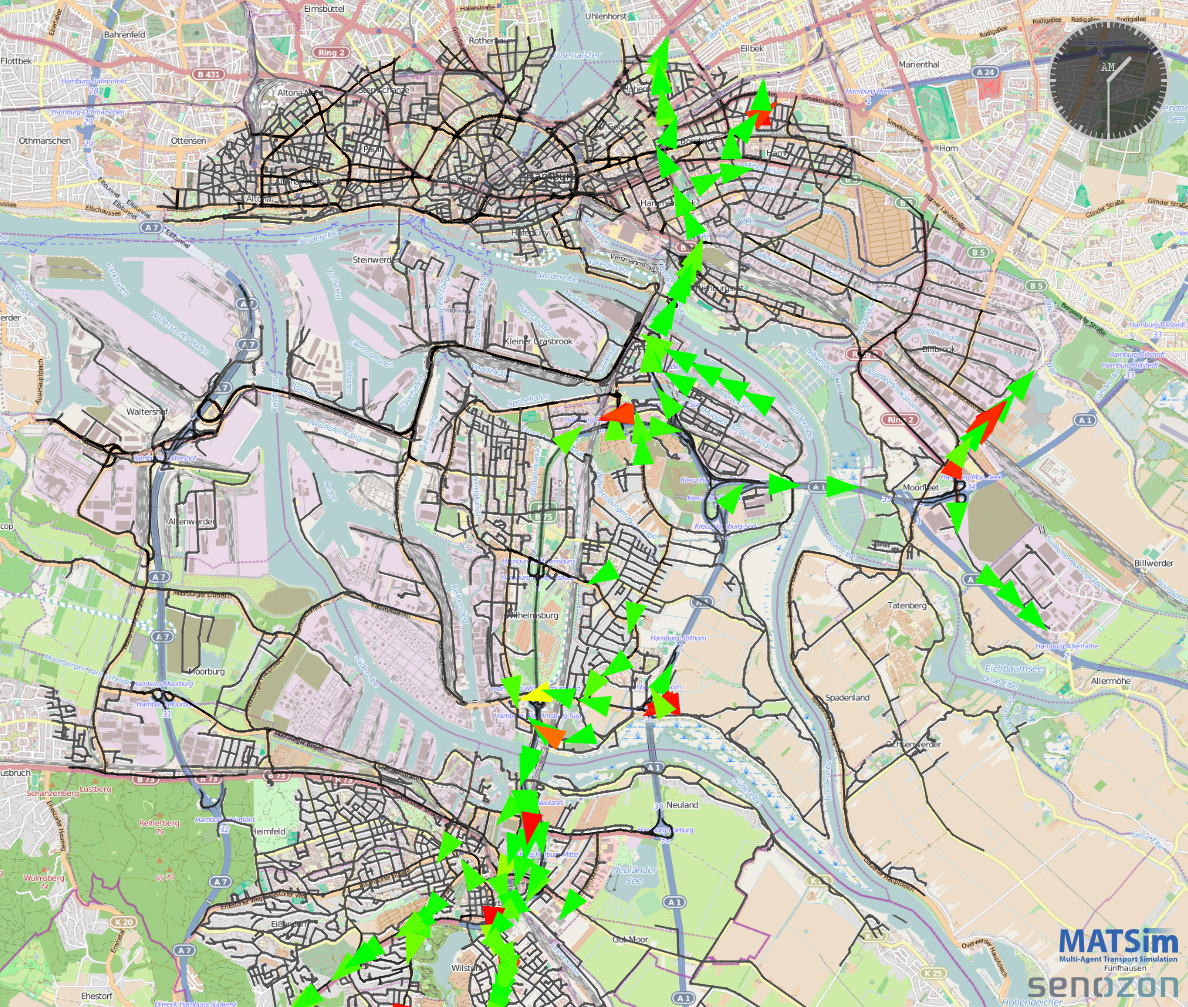
\includegraphics[width=0.7\linewidth]{using/figures/B75iteration20}}%
{}

In summary, the relocation of the highway B75 has no major influence on the overall evacuation time. The evacuation time of about 2\,hours is also within the range of the available safe egress time as described in the previous section. 

Finally, it is of course possible to analyze the results further. The two screenshots above for the situation in iteration 0 at t=3\,hours and for iteration 20 at t=1.5\,hours have been created with senozon Via (the visualizer presented in Chapter~\ref{ch:via}. As a conclusion to this chapter and an illustration for the built-in capabilities of GRIPS for analyzing simulation results, finally the road utilizations of the two variants are shown in Figure~\ref{fig:b75utilization}.
%
\createfigure%
{Network utiliziation for B75}%
{Comparison between network utilization for the old and new track of the B75.}%
{\label{fig:b75utilization}}%
{%
  \createsubfigure%
  {}%
  {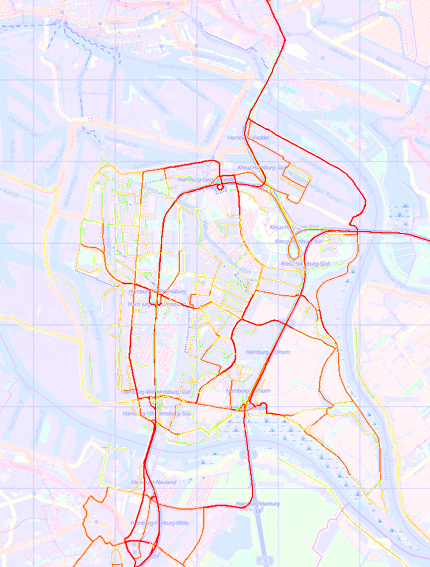
\includegraphics[width=.475\linewidth]{using/figures/b75utilizationold}}%
  {}%
  {}%
  \createsubfigure%
  {}%
  {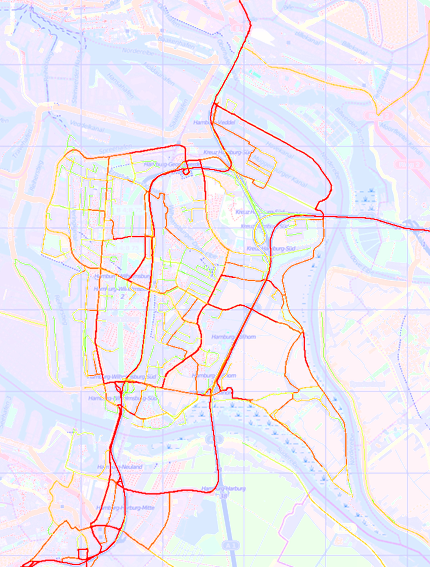
\includegraphics[width=.475\linewidth]{using/figures/b75utilizationnew}}
  {}%
  {}% 
}%
  {}%
% ##################################################################################################################
